\documentclass[a4paper,10pt]{report}
\usepackage[utf8]{inputenc}
\usepackage{graphicx}
\usepackage{titling}

% Title Page
\title{Rendu 2 Projet 2}
\author{Louis Bethune et Jo\"el Felderhoff}
\date{}

\begin{document}
\maketitle

\chapter*{Le programme}

\begin{center}

\includegraphics[scale=0.25]{fouine.jpg} 
\end{center}

\section{Travail effectué}
Voici la liste des parties effectuées pour le rendu
\begin{enumerate}

\item Lexing et parsing du code fouine
\item Interpretation du code fouine :
\begin{enumerate}
	\item Fontionnalités de bases (fonctions, appels de fonctions, addition, structure if then else)
	\item Récursivité
	\item Exceptions
	\item Impératif
	\item Le tout avec une pile d'environnements et des clôtures
	\item Les options de la ligne de commande
	\item Des fichiers test
\end{enumerate}
\item Compilation et exécution vers la SECD : idem que pour l'interprétation
\end{enumerate}

Voici les parties faisant défaut :
\begin{enumerate}
\item L'alternative pour les binômes forts avancés (cela dit je ne suis pas contre m'y consacrer lors des prochains rendus)
\item La gestion des tableaux et des références sur fonctions
\item Les mots clef begin/end
\item Un lexer/parer qui ne pète pas de partout avec des dizaines de conflits
\end{enumerate}

\section{L'exécutable}

L'exécutable s'appelle \textbf{fouine}, et se lance avec \textbf{./fouine}.
Toutes les options de l'énoncé sont prises en compte.  

\begin{enumerate}
\item -debug affiche le programme, et éventuellement le code de la machine à pile (le cas échéant)
\item -machine compile le code pour SECD et l'exécute, cette option se cumule avec la précédente
\item -interm compile le code sans l'exécuter et l'affiche dans un fichier donné en argument, cette option peut se cumuler avec les deux précédentes
\end{enumerate}
  
Plusieurs modes sont disponibles : un mode interactif, lorsque aucun fichier d'entrée n'est spécifié.  
Il suffit alors de taper le programme sur l'entrée, possiblement sur plusieurs lignes. Les déclarations \textbf{let} sans le \textbf{in} peuvent alors être enchaînées, et à la première expression qui ne soit pas une déclaration le programme évalue l'expression. Ce mode interactif est à la "ocaml like".  
  
L'autre mode prend simplement le nom d'une fichier en entrée et l'utilise comme entrée.  
  
La sortie effective du programme interprétée (avec prInt) est préfixée par "stdout of ./fouine :" pour ne pas confondre avce la sortie de ./fouine lui même.  
  
La sortie de ./fouine est la valeur de l'expression parsée, faiblement typée (référence, entier ou clôture).

Vous trouverez des fichiers tests prêts à l'emploi dans le dossier "tests". N'hésitez pas à écrire les vôtres et à soumettre vos mauvaises habitudes d'écriture à notre interpréteur.   

\chapter*{L'interprétation}

\section{Le Lexer/Parser}
Travail commun. Fonctionnel, avec un peu de sucre syntaxique, vous trouverez des exemples de ce qu'on peut faire dans les tests.

Il y a 68 conflits \textit{shift/reduce} et 40 conflits \textit{reduce/reduce}. J'ai (Louis) fait de mon mieux pour les éliminer en m'aidant de l'automate (il y en avait 200 au début) mais je n'ai pas réussi à tout régler. Il résulte de ces tentatives des précédences arbitraires sur certain mots clefs.  

\section{Les fichiers expression.ml et printExpr.ml}
Travail commun. Contient la définition du type Expr, et quelques utilitaires, comme par exemple extraire les variables libres d'une expression.  
  
L'expression parsée est affichée avec des parenthèses supplémentaires afin de lever toute ambiguïté sur les priorités dans l'interprétation des opérateurs.  
  
Un semblant d'indentation automatique a été implémenté pour l'affichage du programme SECD, afin d'en rendre la lecture plus aisée.  
   
\section{L'évaluation de l'expression, sans récursivité}  
Codé par Louis dans eval.ml.  

Il s'agit de l'implémentation proposée en cours. L'expression est évaluée récursivement, en prenant en paramètre l'environnement (par adresse, afin d'éviter les copies).  
  
Les clauses \textbf{let} enrichissent l'environnement en empilant une nouvelle variable, qui peut être associée soit à un entier, soit à une clôture.  
  
La clôture est la donnée de 1) l'expression de la fonction à évaluer et de 2) la partie de l'environnement qui contient les variables libres de l'expression. Cela évite de recopier l'intégralité de l'environnement, au risque de capturer des variables inutiles, et donc améliore les performance.  
  
Lors d'une application de fonction, de la forme \textit{(fun x -> e) y} on enrichit l'environnement de la clôture avec le résultat de l'évaluation de \textit{y}, mappé à l'identificateur \textit{x}, puis on se sert de l'environnement ainsi formé pour évaluer \textit{e}.  
  
\section{La récursivité}  
Codé par Louis.

Même principe que précédemment. Seule la définition de la clôture demande plus de précautions.  
En effet, comme pour une fonction ordinaire on construit un environnement e' pour la clôture, qui contient les variables libres de la fonction. Une fois la clôture construite, on l'ajoute à l'environnement e'. Ainsi la clôture contient un environnement, et en même elle appartient à l'environnement.   
  
Cela ne créée pas de problèmes de boucle infini en pratique, car l'environnement encapsule un pointeur en interne.  
  
Cette situation très compliquée est modélisée en images de synthèse élaborées.  
  
\begin{figure}
\center
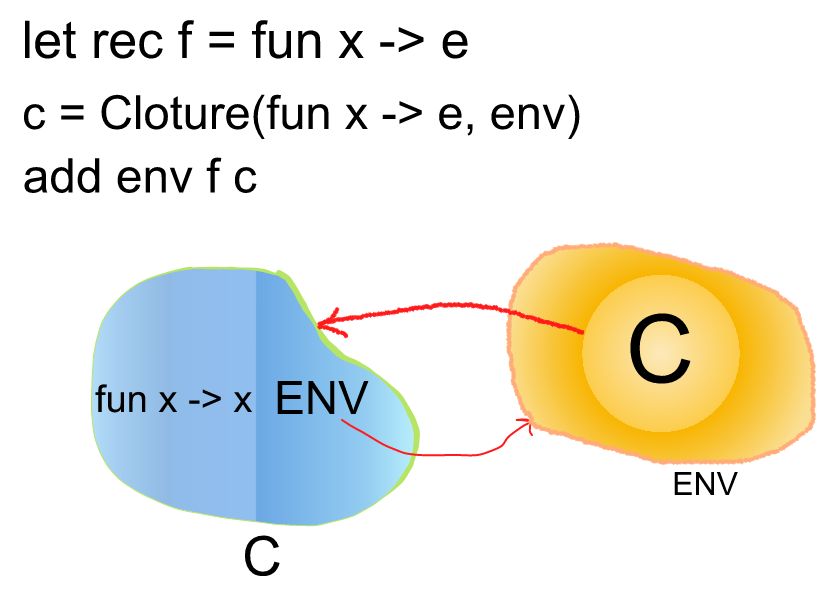
\includegraphics[scale=0.3]{Drawing.png} 
\caption {Phagocytose d'une clôture par une table de hachage}
\end{figure}

\section{Les références et l'impératif}  
Codé par Louis.  
  
En fait c'est une extension qui ne pose pas de problèmes pratiques ou théoriques, elle se traite comme les entiers, c'est juste que les opérations supportés par une référence sont de nature différente.  
  
Notons que cela a également ajouté le ";" pour lequel il convient d'être attentif aux règles de priorité.  

\section{L'environnement et les foncteurs associés}  
Codé par Joël.

\section{Les exceptions et la pile d'environnements}  
Codé par Joël.

\chapter*{La machine SECD}

\begin{center}
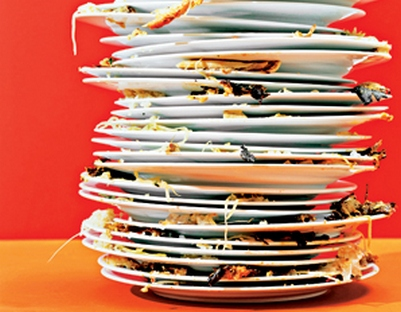
\includegraphics[scale=0.7]{dirty-dishes.jpg} 
\end{center}

\section{La compilation}  
Codé par Louis.

Aucune difficulté technique ici. Compiler vers une machine à pile consiste surtout à afficher les arguments d'un opérateur (quel qu'il soit) avant l'opérateur lui même, et de faire ça récursivement en concaténant les listes d'instructions ainsi obtenues.  
  
Des clôtures sont également utilisées, de manière identique à celles du cas de l'interprétation.  

\section{L'exécution du code compilé}
Codé par Joël.  
\end{document}
